\chapter{Global fits of Parton Distribution Functions} 
As seen in the previous chapter, factorization theorems allow for a separation between contributions 
related to different distance scales: while short distance
effects can be obtained through the computation of partonic matrix elements within perturbation theory, 
long-distance contributions are collected in the universal PDFs $q\left(x,Q^2\right)$. As seen in Sec.~\ref{sec:DGLAP},
knowing the functional form of the PDFs at a given initial scale $Q_0^2$, 
their dependence on the energy scale can be computed by solving the DGLAP evolution equations.
However the dependence on $x$ would be computable only solving QCD in a nonperturbative domain, 
by computing the proton wave function from first principles. We will come back to 
this point in Chapter~\ref{ch:lattice}, when considering lattice QCD observables.
In this Chapter we will discuss the general approach adopted to extract the $x$ dependence of the PDFs
from a discrete set of data, using as basic ingredient the factorization theorems for hadronic observables
discussed before.

%
The general problem is to determine a set of unknown functions given
a collection of data instances. Such kind of task has a long history in data science and AI literature, 
and might be classified as a pattern recognition problem \cite{Forte:2020yip}.
However the specific problem of PDFs determination has some additional peculiarities that we need to keep in mind.
First, PDFs are continuos functions, which makes our problem intrinsically ill-defined, since a continuous real function
$q\left(x,Q_0^2\right)$ cannot be determine from a discrete set of data.
Second, the data are not instances of the functions we are trying to determine, but they are related to 
them through factorization theorems: each point is determined combining a certain subset of PDFs in a non-linear way,
and integrating over a certain range of $x$, as stated in Eq.~\eqref{eq:hadron_hadron}. 
As we will extensively discuss in this and the following chapters,
this fact have several practical and conceptual implications.

%
Another important aspect concerning the problem of PDFs determination 
is the need for results with well quantified uncertainties and correlations.
Universality of PDFs allows one to extract them from a set of data for some specific high-energy processes
and use the result to make predictions for different hadronic observables not included in the analysis.
In order for PDFs to be useful as an input to physics predictions one needs to account for the different
sources of statistical and systematic uncertainties affecting the data entering the analysis, and
propagate them on the resulting PDFs.
Ideally one would like to determine a representation 
of the probability distribution for the unknown PDFs in the whole functional space, so that the full information
about uncertainties and correlations are taken into account when making predictions for new observables.

%
In this chapter we discuss how all these issue have been addressed within the NNPDF collaboration
starting from 2002 \cite{Forte:2002fg}, revising the Monte Carlo replicas generation, the neural networks parameterization
and the minimization procedure. Such methodology has been used to produce the last public NNPDF PDFs set \cite{Ball:2017nwa}
, and a number of studies which will be described in Chapter~\ref{sec:phenomenology} have been performed within the private
{\tt c++ } implementation of this framework.

%
We will then describe how such methodology has been revised and extended 
within the new {\tt n3fit} code, which will be used to produce the next NNPDF release, NNPDF4.0.
In particular, we will discuss in detail the implementation of $\overline{MS}$ PDFs positivity,
the integrability of the nonsinglet sector and the fit basis independence.

\section{NNPDF methodology}

The NNPDF methodology is based on a Monte Carlo determination of the PDFs error, combined
with a neural network parameterization of the unknown PDFs. So far numerical minimization algorithm
have been used, and overfitting has been avoided using a cross-validation technique.
In the first part of this section we revise these general ideas, referring to the baseline {\tt c++} code which
has been used to produce NNPDF3.1. 


\subsection{Monte Carlo PDFs}
As mentioned before, in order to make PDFs sets an useful tool for making predictions,
a faithful estimation of the errors affecting the analysis is necessary. A possible way
to address the problem is to determine the probability distribution of the PDFs set $q\left(x\right)$
given a set of data $D$. Let's denote such probability distribution as $\mathcal{P}\left(q|D\right)$.
A generic observable $\mathcal{O}$ function of one or more PDFs will be determined as an expectation value
over $\mathcal{P}$. Considering for example the case of a DIS observable, the central value and 
uncertainty of the prediction will be given by 
\begin{align}
    \label{eq:expectation_value_observable}
    \langle \mathcal{O}\rangle = \int Dq\, \mathcal{O}\left[q\right] \mathcal{P}\left(q|D\right)\,,\,\,\,\,\,\,\,\,\,
    \text{Var}\left[\mathcal{O}\right] = 
    \int Dq\, \left(\mathcal{O}\left[q\right] - \langle\mathcal{O}\rangle\right)^2
    \mathcal{P}\left(q|D\right)\,.
\end{align}
The problem is then about how to compute a reliable representation of the probability distribution
$\mathcal{P}\left(q|D\right)$.
In the NNPDF framework a Monte Carlo approach is adopted. In this method an ensemble of $N_{rep}$ artificial data is generated
for each experimental point, assuming a multigaussian distribution given by the experimental
covariance matrix. 
More precisely, denoting as $\mathcal{O}^{\text{exp}}_p$ the experimental data for the single point $p$ 
corresponding to the kinematic variables $\{x_p,Q_p^2\}$, 
$N_{rep}$ artificial pseudo-data are generated according to~\cite{Ball:2008by}
\begin{align}
    \mathcal{O}^{(k)}_p = 
    S_{p,N}^{(k)}\,\left(\mathcal{O}^{\text{exp}}_p+\sum_{l=1}^{N_c}r_{p,l}^{(k)}\sigma_{p,l} + r_{p}^{(k)}\sigma_{p, s} \right)\,,
    \,\,\,\,\,\,k = 1,..., N_{rep}
\end{align} 
where
\begin{align}
    S_{p,N}^{(k)} = \prod_{n=1}^{N_a}\left(1 + r_{p,n}^{(k)}\sigma_{p,n}\right)\,,
\end{align}
takes into account normalization errors. 
The variable $\sigma_{p, s}$ represents the uncorrelated statistical uncertainty of the datapoint while 
$\sigma_{p, l}$ and $\sigma_{p, n}$ are the l-th and n-th source of additive and multiplicative systematic uncertainties
respectively. The variables $r_{p}^{(k)}$, $r_{p,l}^{(k)}$ and $r_{p,n}^{(k)}$
are all univariate gaussian random numbers, generating fluctuations of the artificial data around the experimental value.
For each replica $k$, if the l-th additive systematic is correlated between the two experimental points $p$ and $p'$
then $r_{p,l}^{(k)} = r_{p',l}^{(k)}\,$ with an equivalent condition on $r_{p,n}^{(k)}$ to ensure correlation between multiplicative
uncertainties. 
\comment{Check all of this, in the original formula there s an additional term with a square root tat I don t understand.}
$N_{rep}$ independent fits are performed, generating a Monte Carlo ensemble of
PDFs that faithfully reproduces the statistical features of the original experimental 
data, providing the desired representation of the probability density in the space of PDFs.
Central values, uncertainties and correlations can then be computed by doing statistics over
replicas, so that for example
\begin{align}
    \label{eq:expectation_value_observable_mc}
    \langle \mathcal{O}\rangle \sim \frac{1}{N_{rep}}\sum_{k=1}^{N_{rep}}
    \mathcal{O}^{\,(k)}\,,\,\,\,\,\,\,\,\,\,
    \text{Var}\left[\mathcal{O}\right] \sim 
    \frac{1}{N_{rep}}\sum_{k=1}^{N_{rep}}\left(\mathcal{O}^{\,(k)} - \langle\mathcal{O}\rangle\right)^2\,.
\end{align}

The Monte Carlo method therefore propagates the error from the data to the PDFs set
in a natural way, without the need of any assumption on the way error propagation happens.

\subsection{Parameterization and Neural Networks}
As mentioned above, the determination of a continuos function from a discrete set of data 
is an intrinsically ill-defined problem, no matter how copious this set is. In order to overcome this
issue a particular functional form for the $x$ dependence of the PDFs at a reference scale $Q_0$ is chosen,
given in terms of a set of free parameters.
The PDFs at all the other scales $Q$ are determined by solving perturbative evolution equations
and the experimental data are used to determine the optimal values of the free parameters.

%
The choice of the specific parameterization has been largely debated and investigated,
and its final form varies substantially between different fitting groups.
The underlying idea is that the PDFs parameterization has to be flexible enough to describe all the data
entering the analysis without introducing a bias in the final results.
The fact that a too restrictive functional form is likely to introduce a strong bias in the result
has been rapidly recognized, and more and more complex models have been adopted in recent PDFs determinations.

%
The use of neural networks as basic functional form for PDFs was first suggested in 2002 \cite{Forte:2002fg},
in the context of the determination of the DIS structure function $F_2$. 
The idea was further developed in Ref.~\cite{DelDebbio:2004xtd} and applied for the first time to quark
distributions in Ref.~\cite{DelDebbio:2007ee}. This first suggestion was then developed in the context of 
global fits of PDFs by the NNPDF collaboration through a series of intermediate steps 
\cite{Ball:2008by, Ball:2010de, Ball:2012cx, Ball:2014uwa}, the last of which in 2017, with the
release of the PDFs set NNPDF3.1 \cite{Ball:2017nwa}.

%
Neural networks are a class of non-linear maps between some input $\xi_i^{(1)} $ 
and some output $\xi_i^{(L)} $ variables. They are used in several machine learning applications where flexibility
and a lack of bias with respect to a conventional fixed parametrisation  are  desired. 
Like other sets of functions, neural networks, in the limit of an infinite number of parameters, 
can reproduce any differentiable function. The main advantage of using them is the possibility of dealing 
with a greater number of parameters than what is usually available using a more standard parametrization.
The basic element of a neural net is a \textit{neuron} or \textit{node}, which takes a vector $\vec{x} \in \Re^N $ 
as input and gives back a scalar output $ f\left(\vec{x}\right) \in \Re$.
A neural network consists of many neurons stacked into layers and can be graphically represented as a direct graph made by input,
hidden and output layers.
Starting from the input, the output of each layer is used as input for the next one. 
The specific form of the function $f$ characterizing the nodes is usually given by a linear function 
composed with a non linear transformation $g$, called activation function, so that the output of the $i$-th node of 
the $l$-th layer $\xi_i^{(l)}$ is obtained by that of the $(l-1)$-th layer using the relation
\begin{equation}
\label{nodes}
\xi_i^{(l)}= g\left(\sum_jw_{ij}^{(l)}\xi_j^{(l-1)}+\theta_i^{(l)}\right)
\end{equation}
The \textit{weights} $w_{ij}^{(l)} $ and the \textit{biases} $\theta_i^{(l)} $ are the free parameter of the nets, 
to be determined during the fit.
Different choices can be made for the activation function $g$. 
In many cases, including the NNPDF code, it is given by a sigmoid
\begin{equation}
\label{sigmoid}
g\left(x\right)=\frac{1}{1+e^{-x}}
\end{equation}
for the nodes belonging to the hidden layers, and by a linear function $ g(x)=x $ for the output layer.
 
%
Starting from the first proof-of-concepts exercises up to the most recent public release, the basic
neural network architecture employed in all the NNPDF determination has been the same.
The only thing which has been changed is the number of independent parametrized PDFs in a global fit:
five in NNPDF1.0 (up and down quarks and antiquarks), 
seven in NNPDF1.1 (up, down, strange quarks and antiquarks, gluon) and eight in NNPDF3.1
where the total charm PDF was fitted from data for the first time.
Each flavour is independently parameterized using a neural network,
with architecture 2-5-3-1, represented in Fig.~(\ref{nn}). 
The momentum fraction $x$ enters the two input nodes as $x$ and $\log{x}$, followed by two hidden layers with a sigmoid activation function and an output layers with a single node, 
associated with a linear activation function. 
This architecture is supplemented with a preprocessing polynomial factor $x^{-\alpha}\left(1-x\right)^{\beta}$ which controls the PDFs behaviour
at large and small $x$, so that the parameterization for each independent flavour reads
\begin{align}
	\label{eq::paramEvol}
	x\,q_j\left(x, Q_0^2\right) = x^{1-\alpha_{j}}\left(1-x\right)^{\beta_{j}}\text{NN}_{j}\left(x\right)\,.
\end{align}
Eq.~\eqref{eq::paramEvol} can be supplemented by an additional normalization factor $A_j$ which imposes momentum
and valence sum rules. The eight flavours independently parameterized in NNPDF3.1 are 
\begin{align}
    \label{eq:nnpdf31IC_basis}
    q_j = \left[\Sigma, g, V, V_3, V_8, T_3, T_8, c^+ \right]\,,
\end{align} 
with the total charm is defined as $c^+ = c +\bar{c}$.
\begin{figure}[htb]     
	\begin{center}
		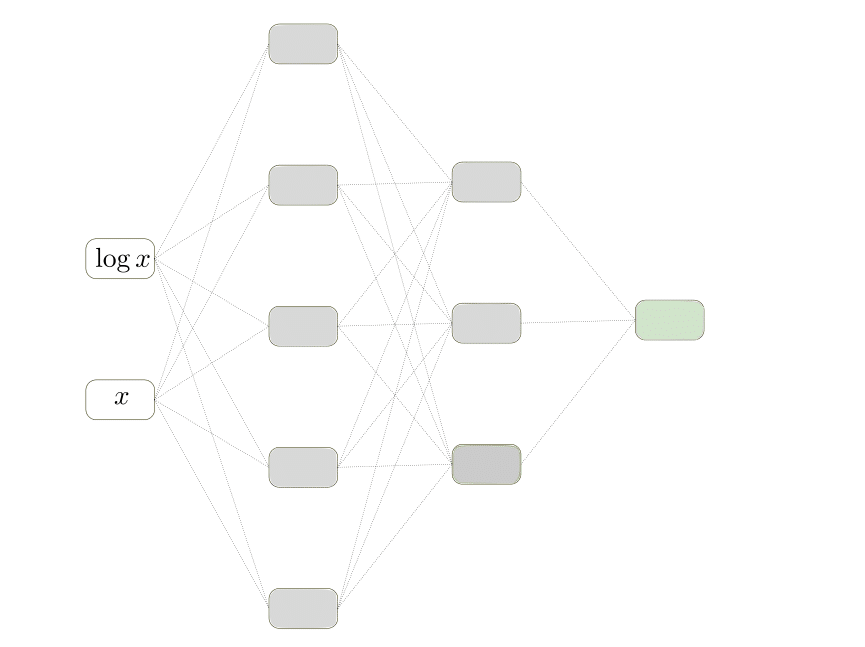
\includegraphics[width=70mm]{nn.png}
	\end{center}
	\caption{Graphical representation of the neural network used in the NNPDF code.}
	\label{nn}                 
\end{figure}
The preprocessing exponents $\alpha_i$ and $\beta_i$ are randomized, by choosing a different value for each replica
within a suitable range. This is determined in a fully self-consistent way: the effective exponents, defined in
Ref.~\cite{Ball:2014uwa} as 
\begin{align}
    \label{eq:effective_exp}
    \alpha_{eff,i}\left(x\right) = \frac{\log q_i\left(x\right)}{\log 1/x}\,, \,\,\,\,
    \beta_{eff,i}\left(x\right) = \frac{\log q_i\left(x\right)}{\log\left(1-x\right)}\,,
\end{align}
are computed for each distribution $q_j$. The $68\%$ confidence level across replicas
is determined for each flavour, and the fit is repeated with the exponents randomized in a range taken equal to twice this 
interval. This procedure is iterated until the range stops changing.

\subsection{Minimization and stopping}
\label{sec:minimization}
The optimal fit is obtained by varying the parameters of $q_j\left(x,Q_0^2\right)$  in such a way that 
some chosen figure of merit is minimized. 
Since the experimental data are assumed to have a multigaussian
distribution, a standard choice for such an object is obtained by taking the standard $\chi^2_k $ for each individual 
dataset $k$
\begin{align}
    \label{eq:chi2}
    \chi^2_k 
    =\sum_{ij}^{N_{dat}}\left(D_{ki}-T_{ki}\right)C_{ij}^{-1}\left(D_{kj}-T_{kj}\right)
\end{align}
and then by building the quantity
\begin{equation}
\label{tot chi2}
\chi^2=\sum_k \chi^2_k
\end{equation}
Here $D_{ki}$ is the i-th experimental data point in the k-th dataset; $T_{ki}$ is the corresponding 
theoretical prediction computed using the corresponding factorization theorem and 
expressed as a function of the free parameters; 
$C_{ij}$ is the covariance matrix, which takes into account both statistical and systematic uncertainties,
as given by the experimental collaborations.
In order to avoid a fitting bias, multiplicative uncertainties required to be handled with a specific method
denoted as $t_0$ prescription, which as been developed in Ref.~\cite{Ball:2009qv} and implemented in all the following
NNPDF PDFs determination.

%
The $\chi^2$ minimization implemented within the NNPDF environment is based on genetic algorithm (GA):
after a first random initialization of the neural network parameters,
the weights are mutated according to a suitable rules, producing
several copies of the original neural net, each one characterized by a different mutation.
Mutations with the lowest value of the figure of merit are selected and the procedure is iterated.
Different variations of GA have been used in every NNPDF PDFs set, including NNPDF3.1.
Another possible option which has been investigated is the CMA algorithm \cite{DBLP:journals/corr/Hansen16a},
which has been used, for example, in a recent NNPDF determination of 
fragmentation functions \cite{Bertone:2017tyb}. As we are going to discuss in the next section,
numerical minimizer are no longer the best possible option. Nowadays several efficient deterministic
methods are available, and an efficient deterministic minimization is more desirable. 

%
Independently from the specific minimization algorithm implemented, overfitting is avoided
employing a cross-validation technique. In this method, the available data are split
in two sets. The first, the training set, is used for the minimization of the error function,
while the second, the validation set, does not enter the fitting procedure. At each iteration of
the minimization algorithm, the error function between the theory predictions from the neural
net and the data is computed for both the training and validation set. At an early stage of
the training, both these quantities are expected to decrease. However, towards the end of the
training, while the error function over the training set will keep decreasing, the same value
computed over the validation data will reach a minimal value, and eventually it may even start
increasing. This is a signal of overfitting, and the point in parameter space yielding the minimal
value of the validation error is the one taken as the fit result.  



\section{The n3fit environment}
\label{sec:n3fit}
The methodology described in the previous section has been completely revised and extended within the new
{\tt n3fit} environment, first presented in \cite{Carrazza:2019mzf}.
In this section we describe the {\tt n3fit} general features, focusing in particular
on the implementation of PDFs positivity and integrability. 
Also we will present some results regarding the problem of the fit basis independence, addressed for the first time
within this environment.

\subsection{Architecture and general structure}
The {\tt n3fit} code is a python-based framework, written using an object-oriented approach and
a number of external libraries. 
Unlike the previous {\tt c++} code of the NNPDF methodology, 
which is fully based on an in-house implementation of neural networks and minimization algorithms,
in the new framework Keras and Tensorflow have been used to deal with them.
This choice greatly simplifies the study of new architectures and techniques recently introduced
in the machine learning literature, allowing for a systematic investigation of many of them, 
and represents an important technological improvement with respect 
to the previous code. 

%
The two main methodological changes in {\tt n3fit} concern the architecture and minimization algorithm:
rather than using eight independent neural networks, each one giving as output a particular flavour, in
the new environment a single net with an eight-dimensional output is used; additionally, gradient descent
methods are implemented to replace the genetic algorithm described before.
The new architecture allow to study and take into account cross-correlations between different PDFs,
while the new gradient descent minimizers have been proved to produce more stable fits than those 
obtained using the genetic algorithm.  

%
For each dataset entering the fit, a vector of $x$ values is given as input to the neural network and,
as in the old methodology, before going through the intermediate layers it is split into $\left(x,\log x\right)$.
The eight output nodes of the neural network provide the eight independent PDFs parameterized at 
the reference scale $Q_0$. We denote such set of independent parton distributions as \textit{fit basis}.
In NNPDF3.1, this is given by Eq.~\eqref{eq:nnpdf31IC_basis}. The new framework allows the user to choose between 
different options: two standard choices are the so called evolution and flavour basis.
While the former represents the equivalent of the one given in Eq.~\eqref{eq:nnpdf31IC_basis}, in
the latter each quark, antiquark and the gluon are independently parameterized. 
The choice of the fit basis should not affect the final results, however different choices might be more
convenient from a methodological point of view, and different architecture setups might be required
when changing the basis. We will extensively discuss these points in Sec.~\ref{sec:fitbasis}.
Depending on our choice for the fit basis, each output can be supplemented with a suitable preprocessing
polynomials, and with normalization factors to impose momentum and valence sum rules.

%
In order to get expressions for physical observables, PDFs have to be
evolved up to the physical scale $Q$ of the hard processes and finally 
combined with partonic matrix elements. These steps happen through two separate convolutions, first with
the evolution kernel which solves DGLAP evolution equations and second with the hard cross sections.
Such convolutions happen by mean of FastKernel tables, introduced and validated in Refs.~\cite{Ball:2010de,Bertone:2016lga}
and used in any subsequent NNPDF analysis.
Each PDFs is projected on a suitable basis functions
\begin{align}
    \label{eq:pdf_interpolation_basis}
    q_i\left(x,Q_0^2\right) = \sum_{\alpha}q_i\left(x_{\alpha},Q_0^2\right)\mathcal{I}^{(\alpha)}\left(x\right) 
\end{align}
so that, considering the case of a DIS observable $\mathcal{O}^{\text{DIS}}$, its final value 
can be expressed as a tensors product of the kind  
\begin{align}
    \label{eq:DIS_obs}
    \mathcal{O}^{\text{DIS}} = \left[\text{FK}\right]_{i\alpha}q_{i\alpha}\,.
\end{align}
with the PDF tensor defined as $q_{i\alpha} = q_i\left(x_{\alpha},Q_0^2\right)$.
The matrix $\text{FK}$, denoted as FK table, stores the precomputed evolution and partonic matrix element 
and can be precomputed for each process entering the analysis.
In the case of hadronic observables $\mathcal{O}^{\text{DY}}$ 
the PDF tensor has to be replaced by a luminosity tensor $\mathcal{L}_{i\alpha j\beta} = q_{i\alpha}q_{j\beta}$ 
and the FK table becomes a rank-4 tensor,
\begin{align}
    \label{eq:DY_obs}
    \mathcal{O}^{\text{DY}} = \left[\text{FK}\right]_{i\alpha j\beta}\mathcal{L}_{i\alpha j\beta}\,.
\end{align}
After computing the value for all the observables entering the fit, the data are split into training and 
validation sets, the $\chi^2$ function of the training set is minimized using gradient descent.
The stopping is implemented according using cross-validation, as described in Sec.~\ref{sec:minimization}.

%
\comment{Add a short paragraph about hyperopt}

\subsection{Fit basis}

\subsection{Positivity}
As recalled in the previous chapter, PDFs are renormalization scheme dependent quantities.
Despite at LO they can be interpreted as probabilities distributions, when considering QCD corrections
such naive picture doesn't hold any more. This in general prevents PDFs from being positive definite objects.
However, independently from the PDFs sign, cross sections for high-energy processes have to be positive.
Such positivity constraint on physical observables might have a non-negligible
impact on the PDFs themself, especially in those kinematic regions where no experimental
data are available: functional forms giving negative cross sections cannot be 
physical solutions of the problem, and therefore should be discarded.  
In the old {\tt c++} code such requirement is implemented through the use of Lagrange multipliers, 
penalizing fit solutions for which a set of chosen high-energy cross sections,
denoted as positivity observables, result to be negative.

%
It would be highly beneficial to work in a renormalization scheme in which PDFs are positive definite
also beyond LO: this would allow to implement directly the positivity of the distributions themself,
without having to rely on a specific choice of positivity observables.
This is indeed the idea of a recent paper~\cite{Candido:2020yat}, where such positive renormalization
scheme for PDFs is built. In the same paper, the Authors work out the relation between such positive
renormalization scheme and the standard $\overline{MS}$, which is the one commonly used in 
PDFs determinations, and surprisingly they find out that NLO $\overline{MS}$ distributions
for quarks, antiquarks and gluon are actually positive definite.  
This result has been accounted for in {\tt n3fit}, where positivity is imposed at the PDFs level.
In the following we describe how this is implemented in the code, and we assess the impact of such constraints
on the large-$x$ region of the PDFs.

\subsection{Integrability}

\subsection{Fit basis independence}
\label{sec:fitbasis}

